\chapter{Forsøg: Sigteanalyse}

\textbf{Apparaturliste}
\begin{itemize}
	\item[-] Sigter med mindst maskevidde på 0,063 mm
	\item[-] Rystemaskine
	\item[-] Vægt med vejenøjagtighed på 0,01 g
	\item[-] Sigtebørste
	\item[-] Skåle i korrosion bestandigt materiale
\end{itemize}
\textbf{Fremgangsmåde}
\newline
Ved en sigteanalyse kan der både udføres en grovsigtning og en finsigtning. Grovsigtningen udføres, hvis materialet vurderes til at have partikler over 16 mm. I dette forsøg er der kun udført en finsigtning, da partiklerne vurderes til at være mindre en 16 mm. Sigtningen er udført på sigter fra 0,063 mm til 2 mm (sigtemålene kan ses i tabellen over resultaterne). 
\newline \indent{     }   Først rengøres hver enkelt sigte forsigtigt med sigtebørste, og herefter samles sigterne forløbende fra den største maskevdde øverst til bunden nederst. Det afmålte materiale hældes på sigten med den største maskevidde på 2 mm, hvorefter sigtetårnet placeres i rystemaskinen og sigtes i 20 minutter.
\newline \indent{     }   Sigteresterne i hver enkelt sigte overføres til skåle og vejes. Hver sigte placeres med bunden opad på et stort stykke papir, og der fejes let på bagsiden, således materialet der sidder fast i maskerne løsnes.
\newline \indent{     }   Alle resultaterne skrives ind i nedenstående tabel, hvor det procentvise gennemfald i hver sigte beregnes ved $gennemfald [\%] = \frac{gennemfald [g]}{samlet prøve [g]}\cdot 100 [\%]$. Herefter optegnes en sigtekurve over resultaterne med det procentvise gennemfald af y-aksen i aritmisk skala, og kornstørrelse af x-aksen i logaritmisk skala. Herpå aflæses de to punkter der ligger mellem henholdsvis 10\% og 60\%, og der laves lineær regression imellem de to punkter. Herudfra kan 10\%-fraktilen, $d_{10}$, og 60\%-fraktilen, $d_{60}$, beregnes. Disse bruges til at udregne uensformighedstallet $U = \frac{d_{60}}{d_{10}}$
\newline
\newline
\textbf{Resultater}
\newline
\newline
Forsøget er udført to gange. I Figur \ref{fig:forsoget} og Figur \ref{fig:forsogto} ses en oversigt over de resultater der er opnået i hvert forsøg. 

\begin{figure}[htbp] \centering
	\begin{minipage}[b]{0.48\textwidth}\centering
		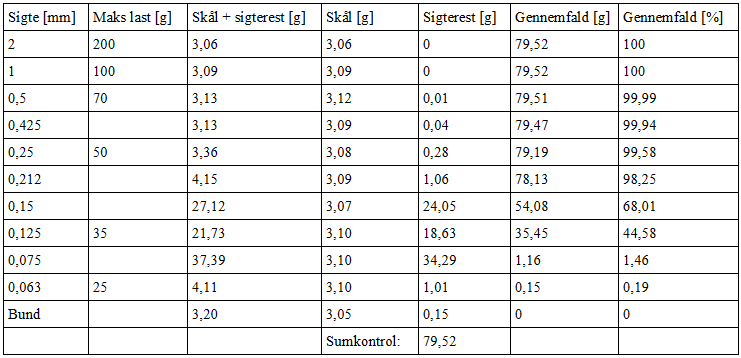
\includegraphics[width=1.7\textwidth]{billeder/forsogetsigteanalyse.png}
		\caption{Tabel over resultater for det første udførte forsøg}
		\label{fig:forsoget}
	\end{minipage}\hfill
\end{figure}

\begin{figure}[htbp] \centering
	\begin{minipage}[b]{0.48\textwidth}\centering
		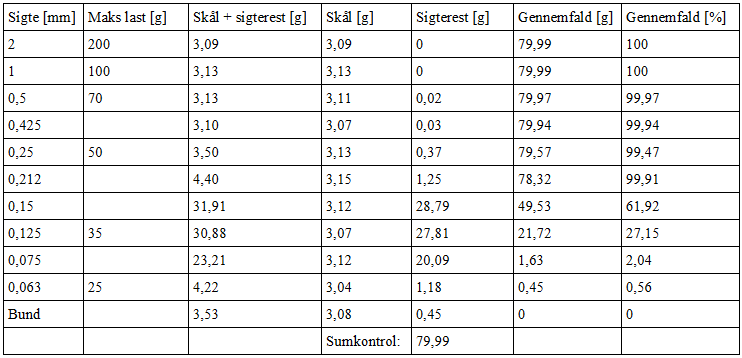
\includegraphics[width=1.7\textwidth]{billeder/forsogtosigteanalyse.png}
		\caption{Tabel over resultater for det andet udførte forsøg}
		\label{fig:forsogto}
	\end{minipage}\hfill
\end{figure}

\textbf{Beregninger}
\newline
\underline{Forsøg 2}
\newline
\newline
60\%-fraktilen og 10\%-fraktilen beregnet, ved at lave lineær regression imellem sigte med maskestørrelse $0,\!125$ mm og $0,\!15$ mm, der ligger mellem henholdsvis 60\% og 10\% i sigtekurven. 
\newline
\newline
Nedenstående ligning fås ved 10\%-fraktilen:
\begin{center}
	$y = 502,\!31x - 35,\!635 \leftrightarrow d_{10}=0,\!091$
\end{center}

Nedenstående ligning fås ved 60\%-fraktilen:
\begin{center}
	$y = 1390,\!7x - 146,\!68 \leftrightarrow d_{60}=0,\!15$
\end{center}

Uensformighedstallet beregnes til:
\begin{center}
	$U=\frac{d_{60}}{d_{10}} = \frac{0,\!15}{0,\!091} = 1,\!64$
\end{center}

\textbf{Fejlkilder}
\newline
Sigteresterne kan ikke være børstet helt ud af maskerne, og alt materialet bliver dermed ikke vejet med. Derudover er det muligt, at sigterne ikke er blevet børstet grundigt nok inden forsøgsstart, og der kan dermed sidde materiale fra anden prøve i maskerne, der bliver vejet med.
\newline
Noget materiale kan være gået tabt under processen, idet partiklerne er meget små. 